\documentclass{book}

\usepackage{float} % Required for specifying the exact location of a figure or table
\usepackage{graphicx} % Required for including images
\usepackage{wrapfig}
\newcommand{\HRule}{\rule{\linewidth}{0.5mm}} % Command to make the lines in the title page

\setlength\parindent{0pt} % Removes all indentation from paragraphs
%\setcounter{tocdepth}{2}
\graphicspath{ {.././source/} }

\begin{document}


\section{Using COGO Tools in QGIS}
%\pagebreak

\subsection{Set up the Azimuth and Distance Plugin \small(Azd Plugin).}
%\paragraph{After starting QGIS in the basemap}

\subsubsection{Launch Azd Plugin}
\large {In the Plugins drop down(1) under the topography group select the Azd Plugin(2)(see fig.).}
\begin{figure}[H] % included image
\begin{center}
%\centering
	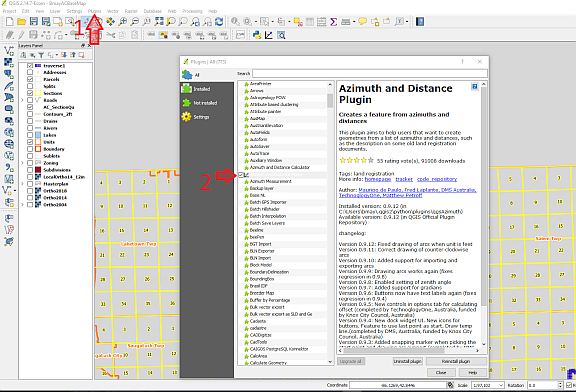
\includegraphics[scale=.25]{1.png}
	\end{center}
	\caption{launch plugin}	
\end{figure}
%\pagebreak
\clearpage

\subsubsection{Configure Active Layer}
\large Note here which layer is active.
\begin{figure}[H] % included image
\begin{center}
	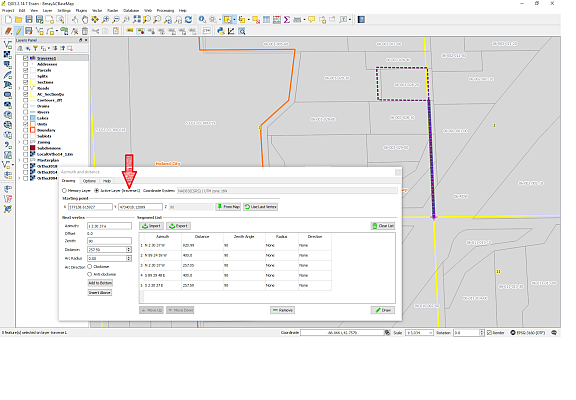
\includegraphics[scale=.2]{2.png} 
	\end{center}
	\caption{check active layer}
\end{figure}

%\noindent
If necessary, left click the layer traverse 1 in Layer Panel to activate it(see fig.).
\begin{figure}[H] % Example of including images
\begin{center}
	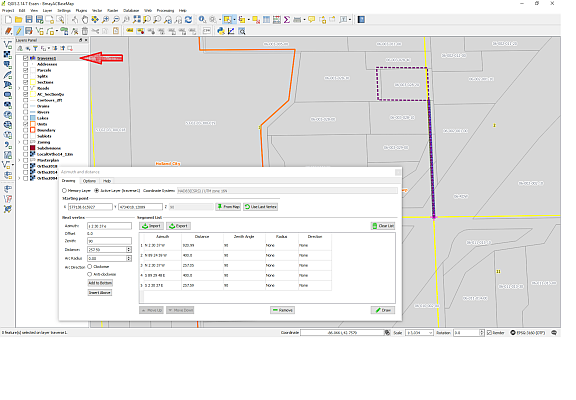
\includegraphics[scale=.2]{3.png} 
	\end{center}
	\caption{activate layer}
\end{figure}

\subsubsection{Configure Options}
\large On Options Tab: Select Boundary, Bearing, Feet, and Degree radio buttons.
\begin{figure}[H]
\begin{center}
	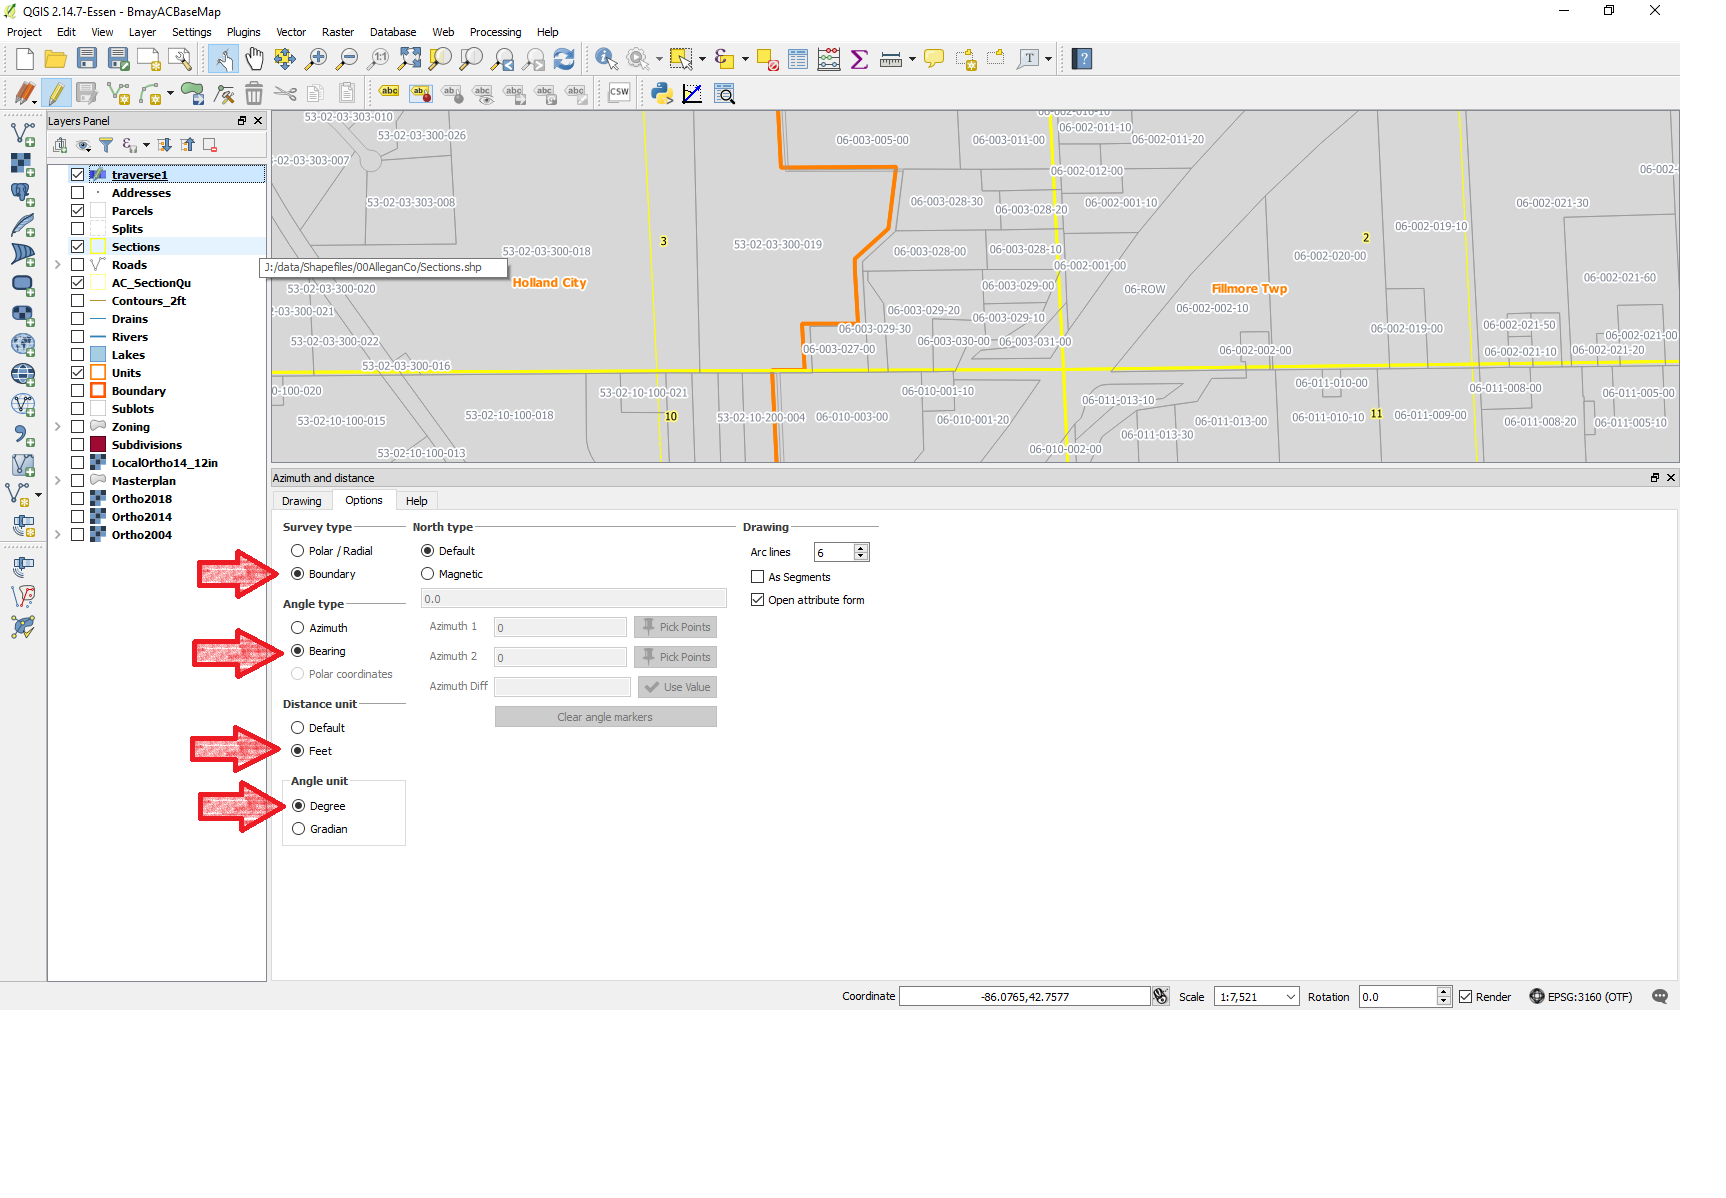
\includegraphics[scale=.3]{4.png} 
	\end{center}
	\caption{Plugin Options}
\end{figure}
\pagebreak

\subsubsection{Using the tool}
\large Boundary descriptions are entered into the Drawing Tab. Azimuth (bearing) and Distance are the important boxes (Set Offset = 0 and Zenith = 90 and ignore)(see below).
\begin{figure}[H]
\begin{center}
	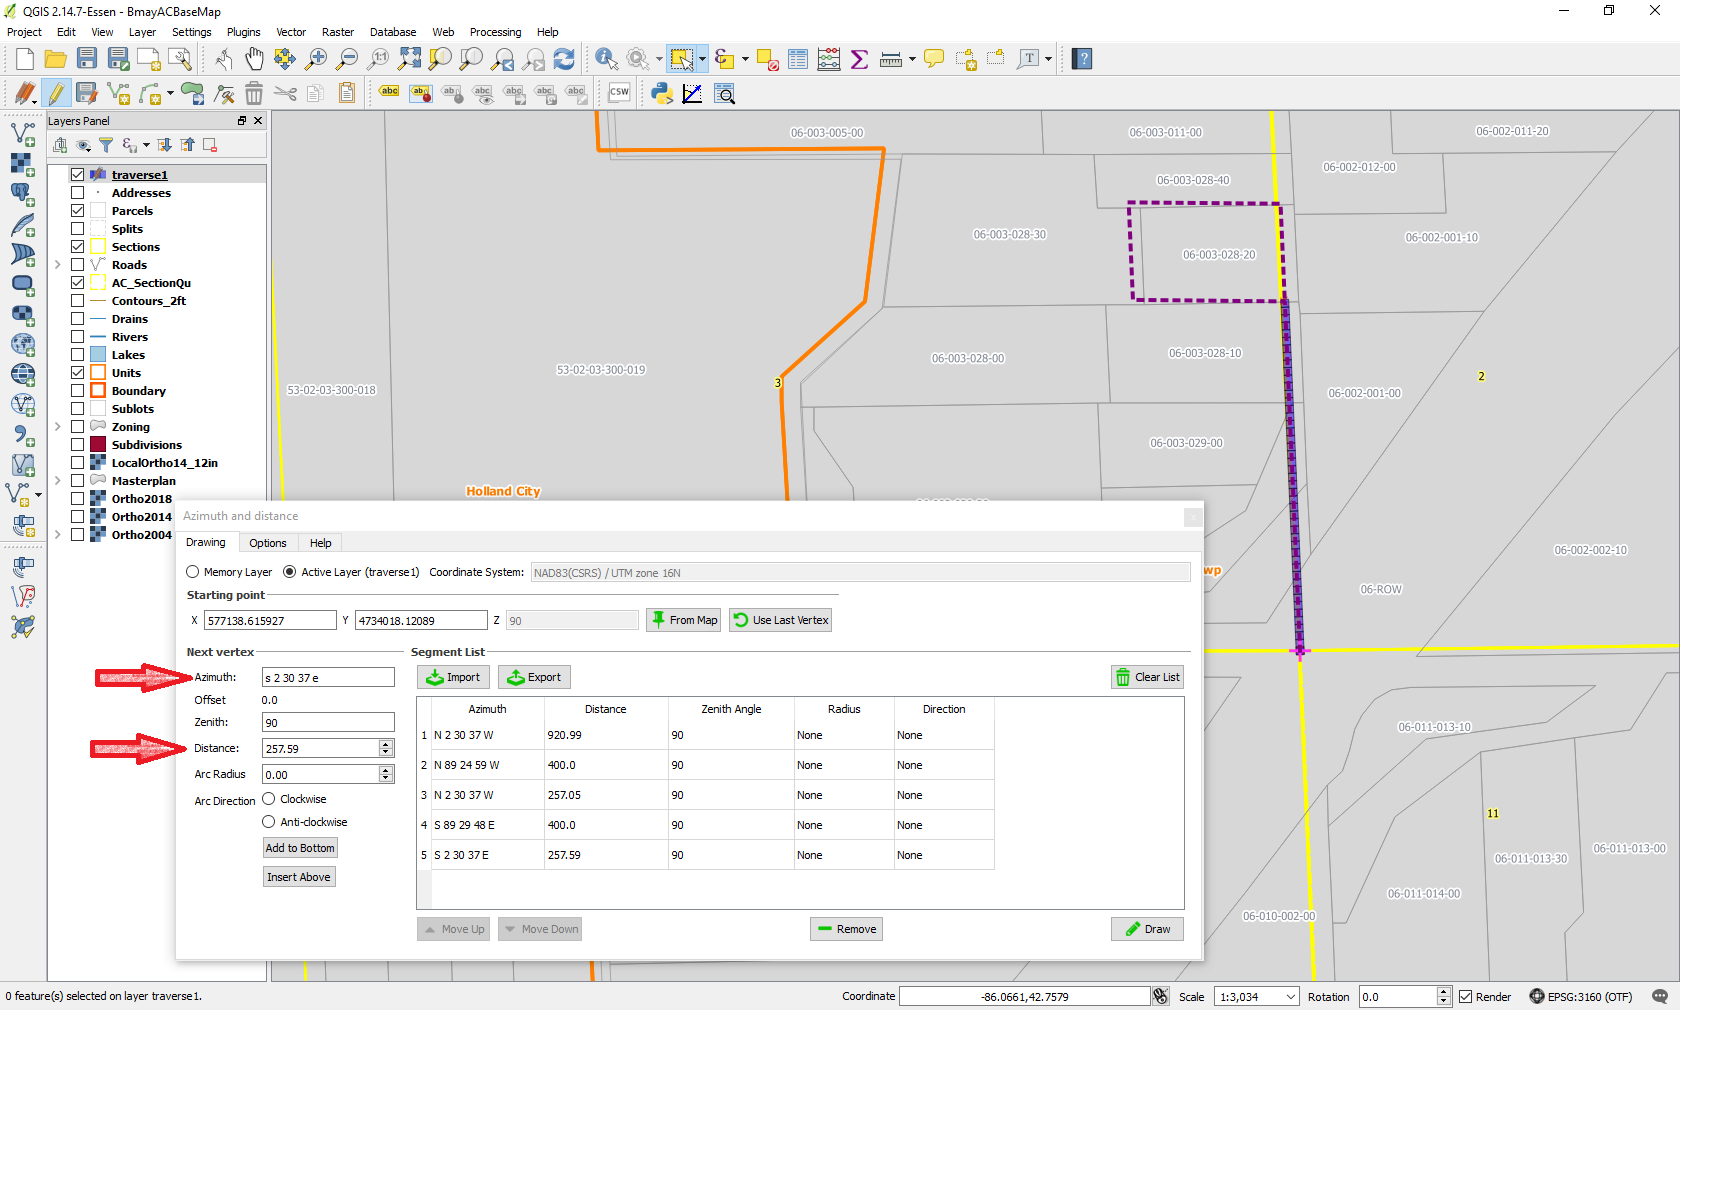
\includegraphics[scale=.3]{5.png} 
	\end{center}
	\caption{Entering Bounds}
\end{figure}
\pagebreak

\subsection{Configure editing environment}
\large Use Settings Dropdown and Snapping Options to enable snapping to Sections, Quarter Sections, and or Parcels if desired (see fig.).

\begin{figure}[H]
\begin{center}
	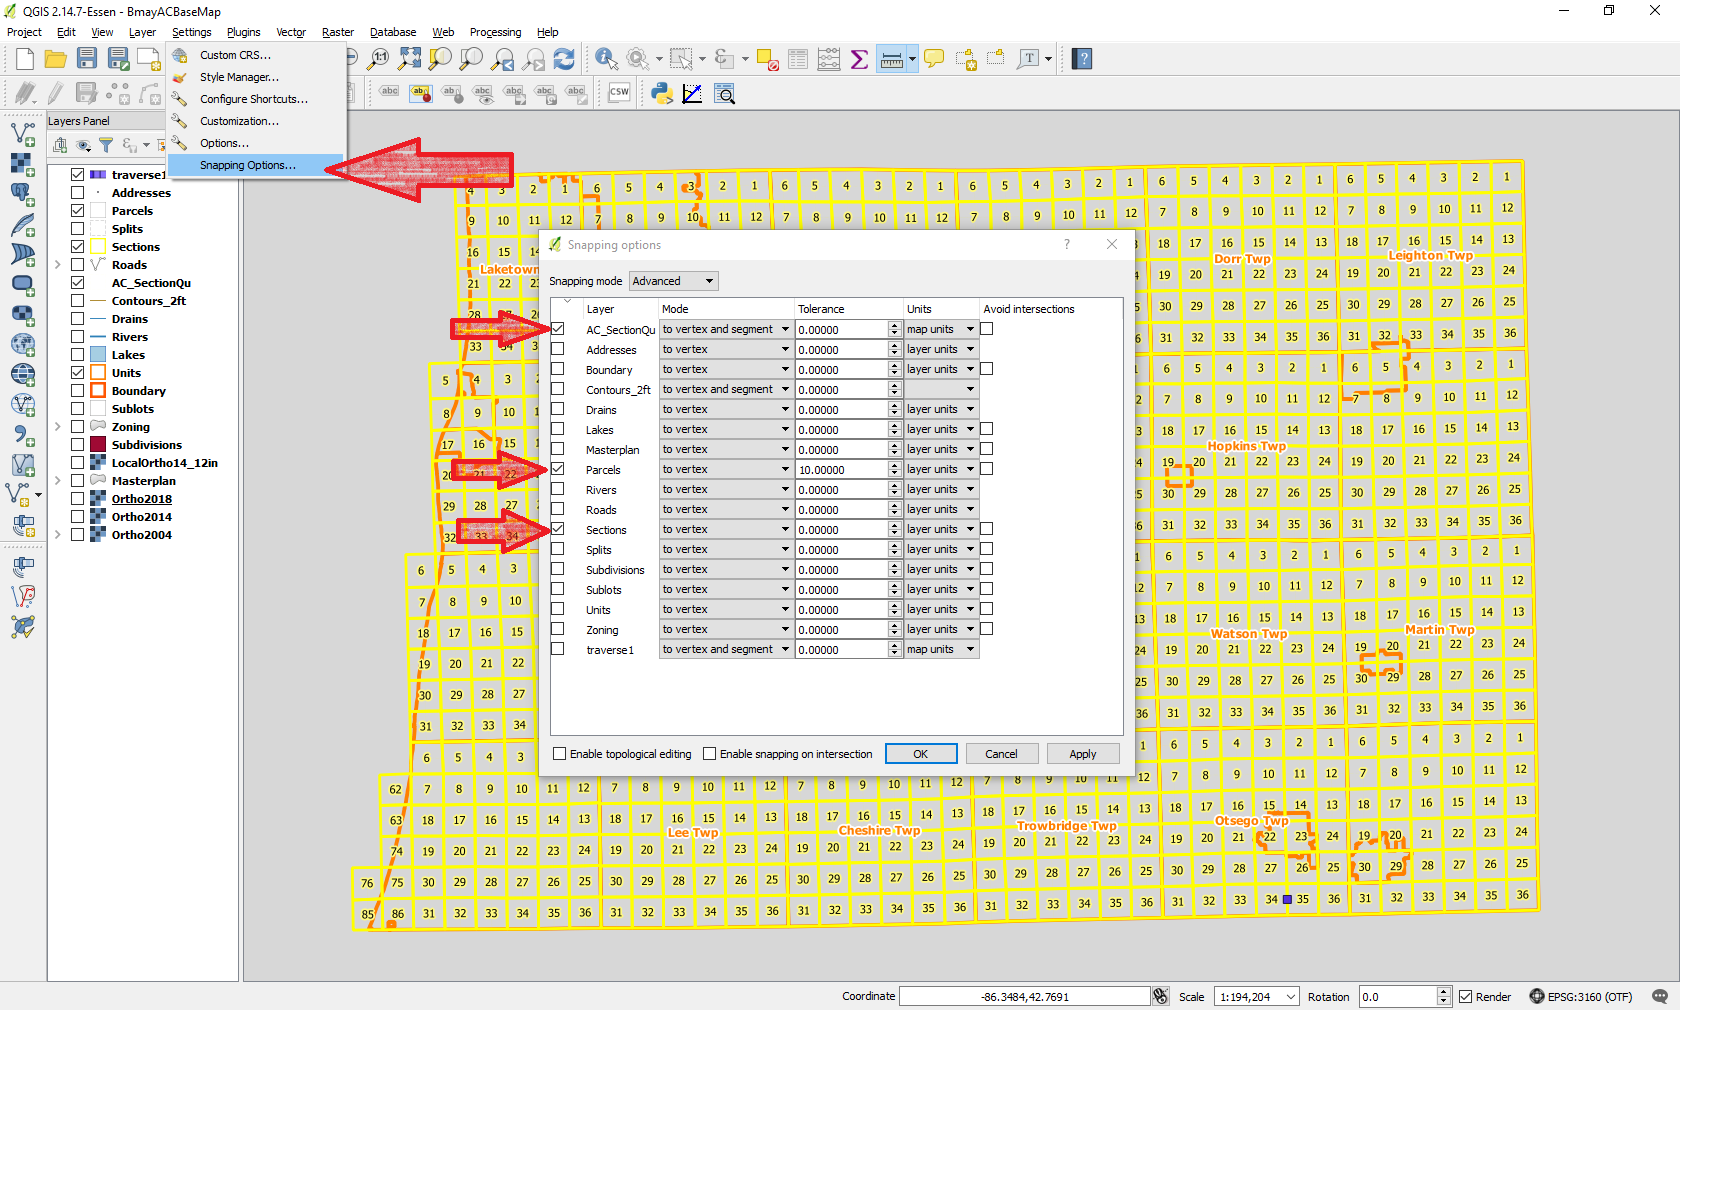
\includegraphics[scale=.3]{7.png} 
	\end{center}
	\caption{Configure editing environment}
\end{figure}
\pagebreak

\subsection{Locate Point of Commencement}
To get to the Point of Commencement,
\medskip

Use \textbf{any combination} of the following methods:
\begin{itemize}
	\item{Using Reference Layer}
	\item{Using Measuring Tool}
	\item{Search by Parcel Number \small(Search Layers Plugin)}
	\item{Draw COGO lines \small(Azd Plugin)}
\end{itemize}

\subsubsection{Using Reference Layer}

{\large Use reference layers; Units, AC\_SectionsQu, Sections, and Parcels.  Toggle layers on and off in Layers Panel and zoom in and out with mouse wheel.}
\pagebreak

\subsubsection{Using Measuring Tool}
\large Use the measuring tool, make sure to set units to feet.  To exit current measurement right click (see fig.).

\end{document}